\documentclass[12pt]{article}
\usepackage[a4paper, margin=1in]{geometry} 
\usepackage{graphicx} 
\usepackage{hyperref}
\usepackage{float}
\usepackage{multicol}
\usepackage{multirow}
\usepackage{amsmath}
\usepackage[ruled]{algorithm2e}
\usepackage{amssymb}
\usepackage[font=small, labelfont=bf]{caption}
\usepackage[table,xcdraw]{xcolor}

\title{Lecture Notes for \\ INF281 Basics of Bioinformatics Sequence Analysis}
\author{Takaya Saito}
\date{}

\begin{document}

\pagenumbering{arabic}
\setcounter{page}{94}

\makeatletter 
\renewcommand{\thefigure}{\arabic{section}.\arabic{figure}}
\renewcommand{\thetable}{\arabic{section}.\arabic{table}}
\makeatother

%
% Hidden Markov model
%
\setcounter{section}{12}
\setcounter{figure}{0}
\setcounter{table}{0}
\section{Hidden Markov model}
%\documentclass[12pt]{article}
%\usepackage[a4paper, margin=1in]{geometry} 
%\usepackage{graphicx} 
%\usepackage{hyperref}
%\usepackage{float}
%\usepackage{multicol}
%\usepackage{multirow}
%\usepackage{amsmath}
%\usepackage[font=small, labelfont=bf]{caption}
%
%\begin{document}

%
% Hidden Markov model
%
\subsection{Hidden Markov model}
An HMM (hidden Markov model) is a probabilistic graphical model that assumes a Markov property. It contains two different types of probabilities: transition and emission probabilities.

\begin{figure}[H]
  \centering
      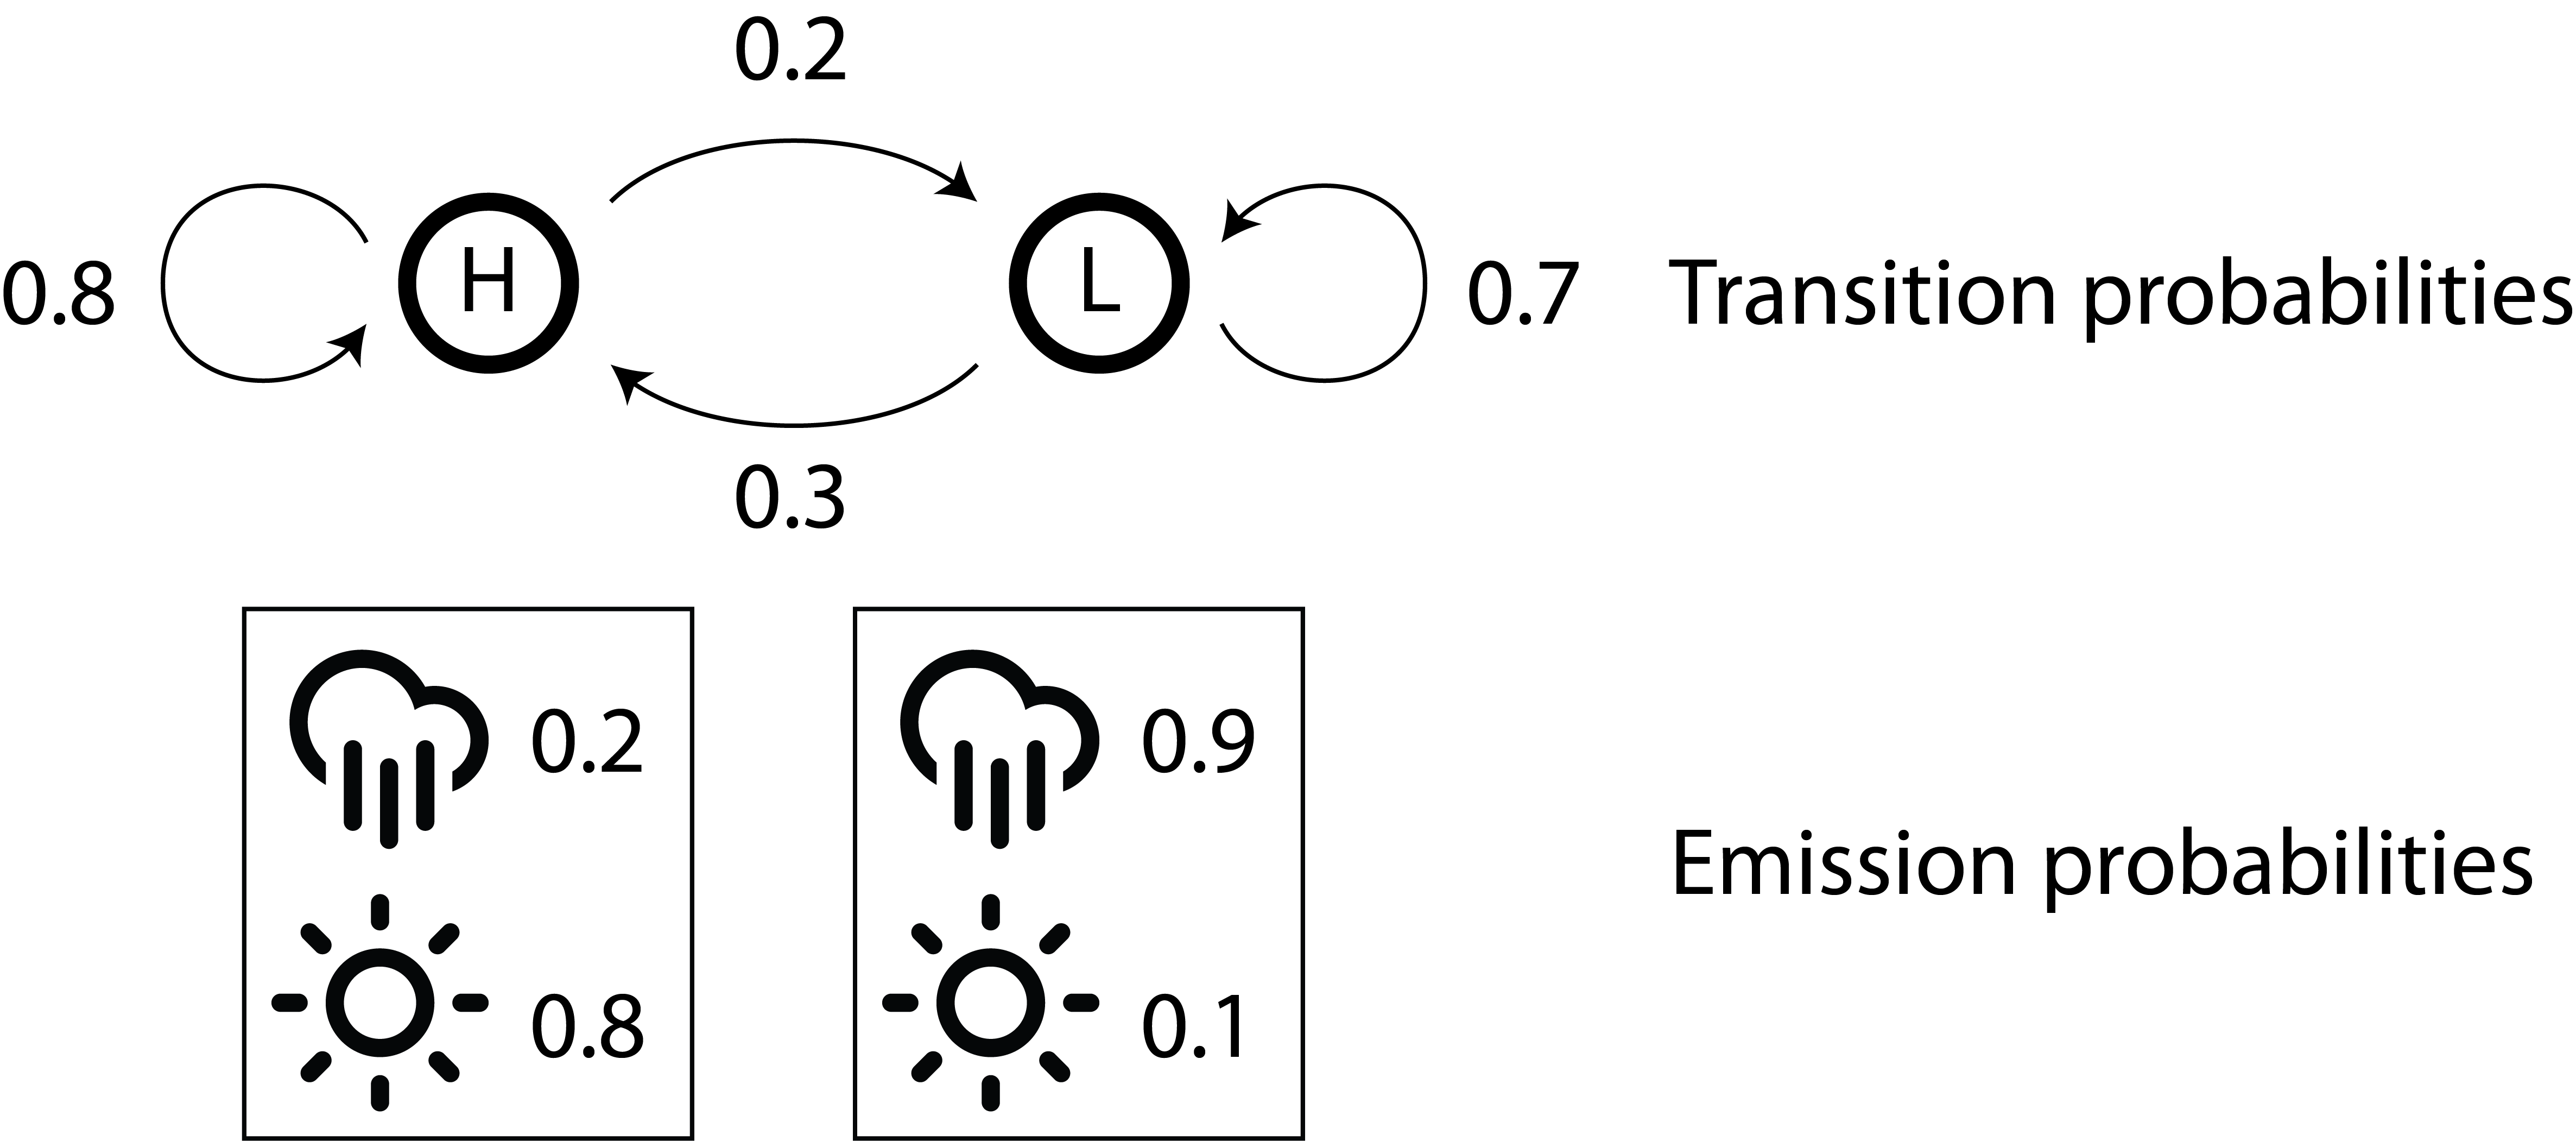
\includegraphics[width=0.5 \textwidth]{fig13/HMM_example.png}
  \caption{HMM for weather conditions}
\end{figure}

%
% Example of HMM probability calculation
%
\subsubsection*{Example of HMM probability calculation}
Calculate the probability when the observed weather conditions are (Sunny, Sunny, Sunny) and the corresponding states are (L, H, H). Assume no particular prior distribution for the initial states. \\

$\begin{aligned}
&p(\mathrm{L}) \cdot  p(\mathrm{Sunny}|\mathrm{L}) 
\times p(\mathrm{H}|\mathrm{L}) \cdot  p(\mathrm{Sunny}|\mathrm{H}) 
\times p(\mathrm{H}|\mathrm{H}) \cdot  p(\mathrm{Sunny}|\mathrm{H}) \\
&= 0.5 \cdot 0.1 \times 0.3 \cdot 0.8 \times 0.8 \cdot 0.8 \\
&= 0.00768
\end{aligned} $

%
% Search and training of HMM
%
\subsubsection*{Search and training of HMM}
A dynamic programming is commonly used to search the most probable path, and an EM (Expectation-Maximization) algorithm is often used for training.

\begin{itemize}
\item Viterbi algorithm: A dynamic programming for searching HMM
\item Baum–Welch algorithm: An EM algorithm for training HMM
\end{itemize}

%
% Exercise \thesection.1
%
\subsubsection*{Exercise \thesection.1}
Use the transition and emission probabilities in the HMM above and calculate the probability when the observed weather conditions are (Rain, Rain, Sunny) and the corresponding states are (H, L, L). 

\bigskip 

\bigskip 

%\end{document}

%\documentclass[12pt]{article}
%\usepackage[a4paper, margin=1in]{geometry} 
%\usepackage{graphicx} 
%\usepackage{hyperref}
%\usepackage{float}
%\usepackage{multicol}
%\usepackage{multirow}
%\usepackage{amsmath}
%\usepackage[font=small, labelfont=bf]{caption}
%
%\begin{document}

%
% Viterbi algorithm
%
\subsection{Viterbi algorithm}
The Viterbi algorithm is used to find the most probable path of HMM.

%
% Probabilities of possible paths when the states are unknown
%
\subsubsection*{Probabilities of possible paths when the states are unknown}
All possible paths need to be considered for an observed instance when the states are unknown. 

%
% Example of all possible paths
%
\subsubsection*{Example of all possible paths}
How many possible paths can one find when there are two states \{S1, S2\} and three observation \{O1, O2, O3\}? \\

\noindent
The number of all possible paths: 8 \\
(S1, S1, S1), (S1, S1, S2), (S1, S2, S1), (S1, S2, S2), \\
(S2, S1, S1), (S2, S1, S2), (S2, S2, S1), (S2, S2, S2)

%
% Dynamic programming
%
\subsubsection*{Dynamic programming}
The Viterbi algorithm is a dynamic programming that can be used to find the most probable path and its probability of an HMM.

%
% Example of dynamic programming
%
\subsubsection*{Example of dynamic programming}
\begin{figure}[H]
  \centering
      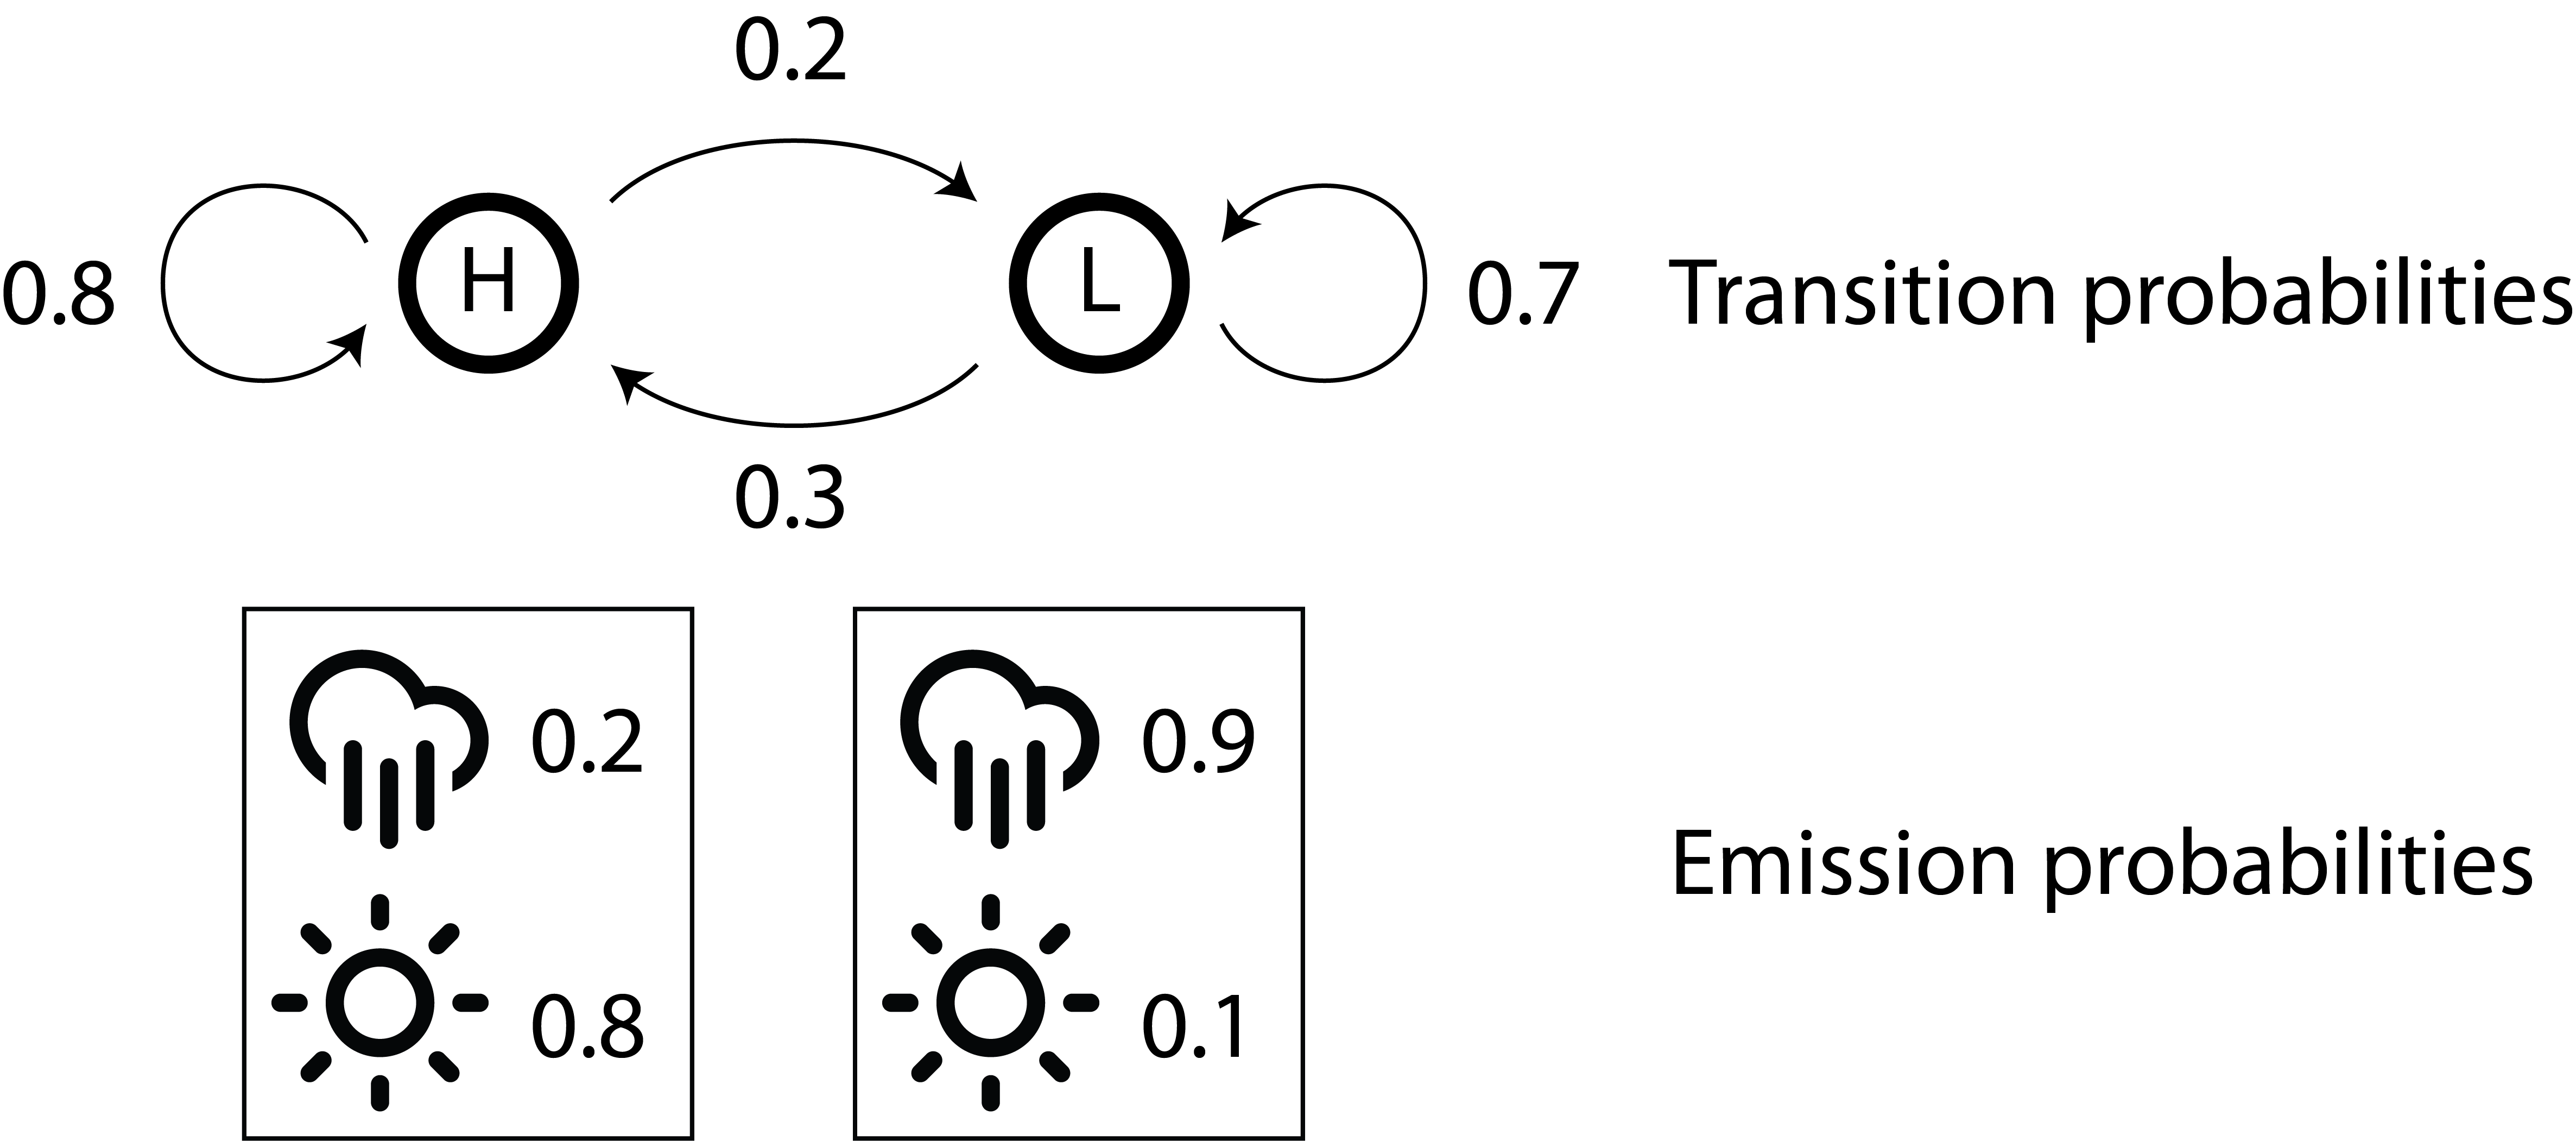
\includegraphics[width=0.5 \textwidth]{fig13/HMM_example.png}
  \caption{HMM for weather conditions}
\end{figure}

Find the most probable path in the HMM above when the observed weather conditions are (Sunny, Sunny, Sunny). Assume no particular prior distribution for the initial states.

\begin{table}[H]
\centering
\caption{DP table for the Viterbi algorithm}
\label{my-label}
\begin{tabular}{|c|l|l|}
\hline
                       & \multicolumn{1}{c|}{H}     & \multicolumn{1}{c|}{L}     \\ \hline
Sunny                  & $0.5 \times 0.8 = \textbf{0.4}$              & $0.5 \times 0.4 = 0.2$              \\ \hline
\multirow{2}{*}{Sunny} & (H)$0.4 \times 0.8 \times 0.8 = \textbf{0.256}$     & (H)$0.4 \times 0.2 \times 0.1 = 0.008$     \\
                       & (L)$0.2 \times 0.3 \times 0.8 = 0.048$     & (L)$0.2 \times 0.7 \times 0.1 = 0.014$     \\ \hline
\multirow{2}{*}{Sunny} & (H)$0.256 \times 0.8 \times 0.8 = \textbf{0.16384}$ & (H)$0.256 \times 0.2 \times 0.1= 0.00512$  \\
                       & (L)$0.014 \times 0.3 \times 0.8 = 0.00336$ & (L)$0.014 \times 0.7 \times 0.1 = 0.00098$ \\ \hline
\end{tabular}
\end{table}

%
% Exercise \thesection.2
%
\subsubsection*{Exercise \thesection.2}
Use the HMM above and find the most probable path for the following weather conditions. Assume no particular prior distribution for the initial states.

\begin{enumerate}
\item (Sunny, Rain).
\begin{table}[H]
\centering
\begin{tabular}{|c|c|c|}
\hline
      & H & L \\ \hline
Sunny & \quad \quad \quad \quad  \quad \quad \quad \quad &  \quad \quad \quad \quad \quad \quad \quad \quad \\ \hline
Rain  &   &    \\ \hline
\end{tabular}
\end{table}

\item (Rain, Rain).
\begin{table}[H]
\centering
\begin{tabular}{|c|c|c|}
\hline
      & H & L \\ \hline
Rain & \quad \quad \quad \quad  \quad \quad \quad \quad &  \quad \quad \quad \quad \quad \quad \quad \quad \\ \hline
Rain  &   &    \\ \hline
\end{tabular}
\end{table}

\end{enumerate}

\bigskip 

%\end{document}

%\documentclass[12pt]{article}
%\usepackage[a4paper, margin=1in]{geometry} 
%\usepackage{graphicx} 
%\usepackage{hyperref}
%\usepackage{float}
%\usepackage{multicol}
%\usepackage{multirow}
%\usepackage{amsmath}
%\usepackage[table,xcdraw]{xcolor}
%\usepackage[font=small, labelfont=bf]{caption}
%
%\begin{document}

%
% HMM profile
%
\subsection{HMM profile}
An HMM (Hidden Markov model) profile is similar to a regular profile, but it is based on a probabilistic graphical model.

%
% HMM profile to find local alignments
%
\subsubsection*{HMM profile to find sub-strings}
An HMM profile represents position-specific probabilities of amino acids.

\begin{figure}[H]
  \centering
      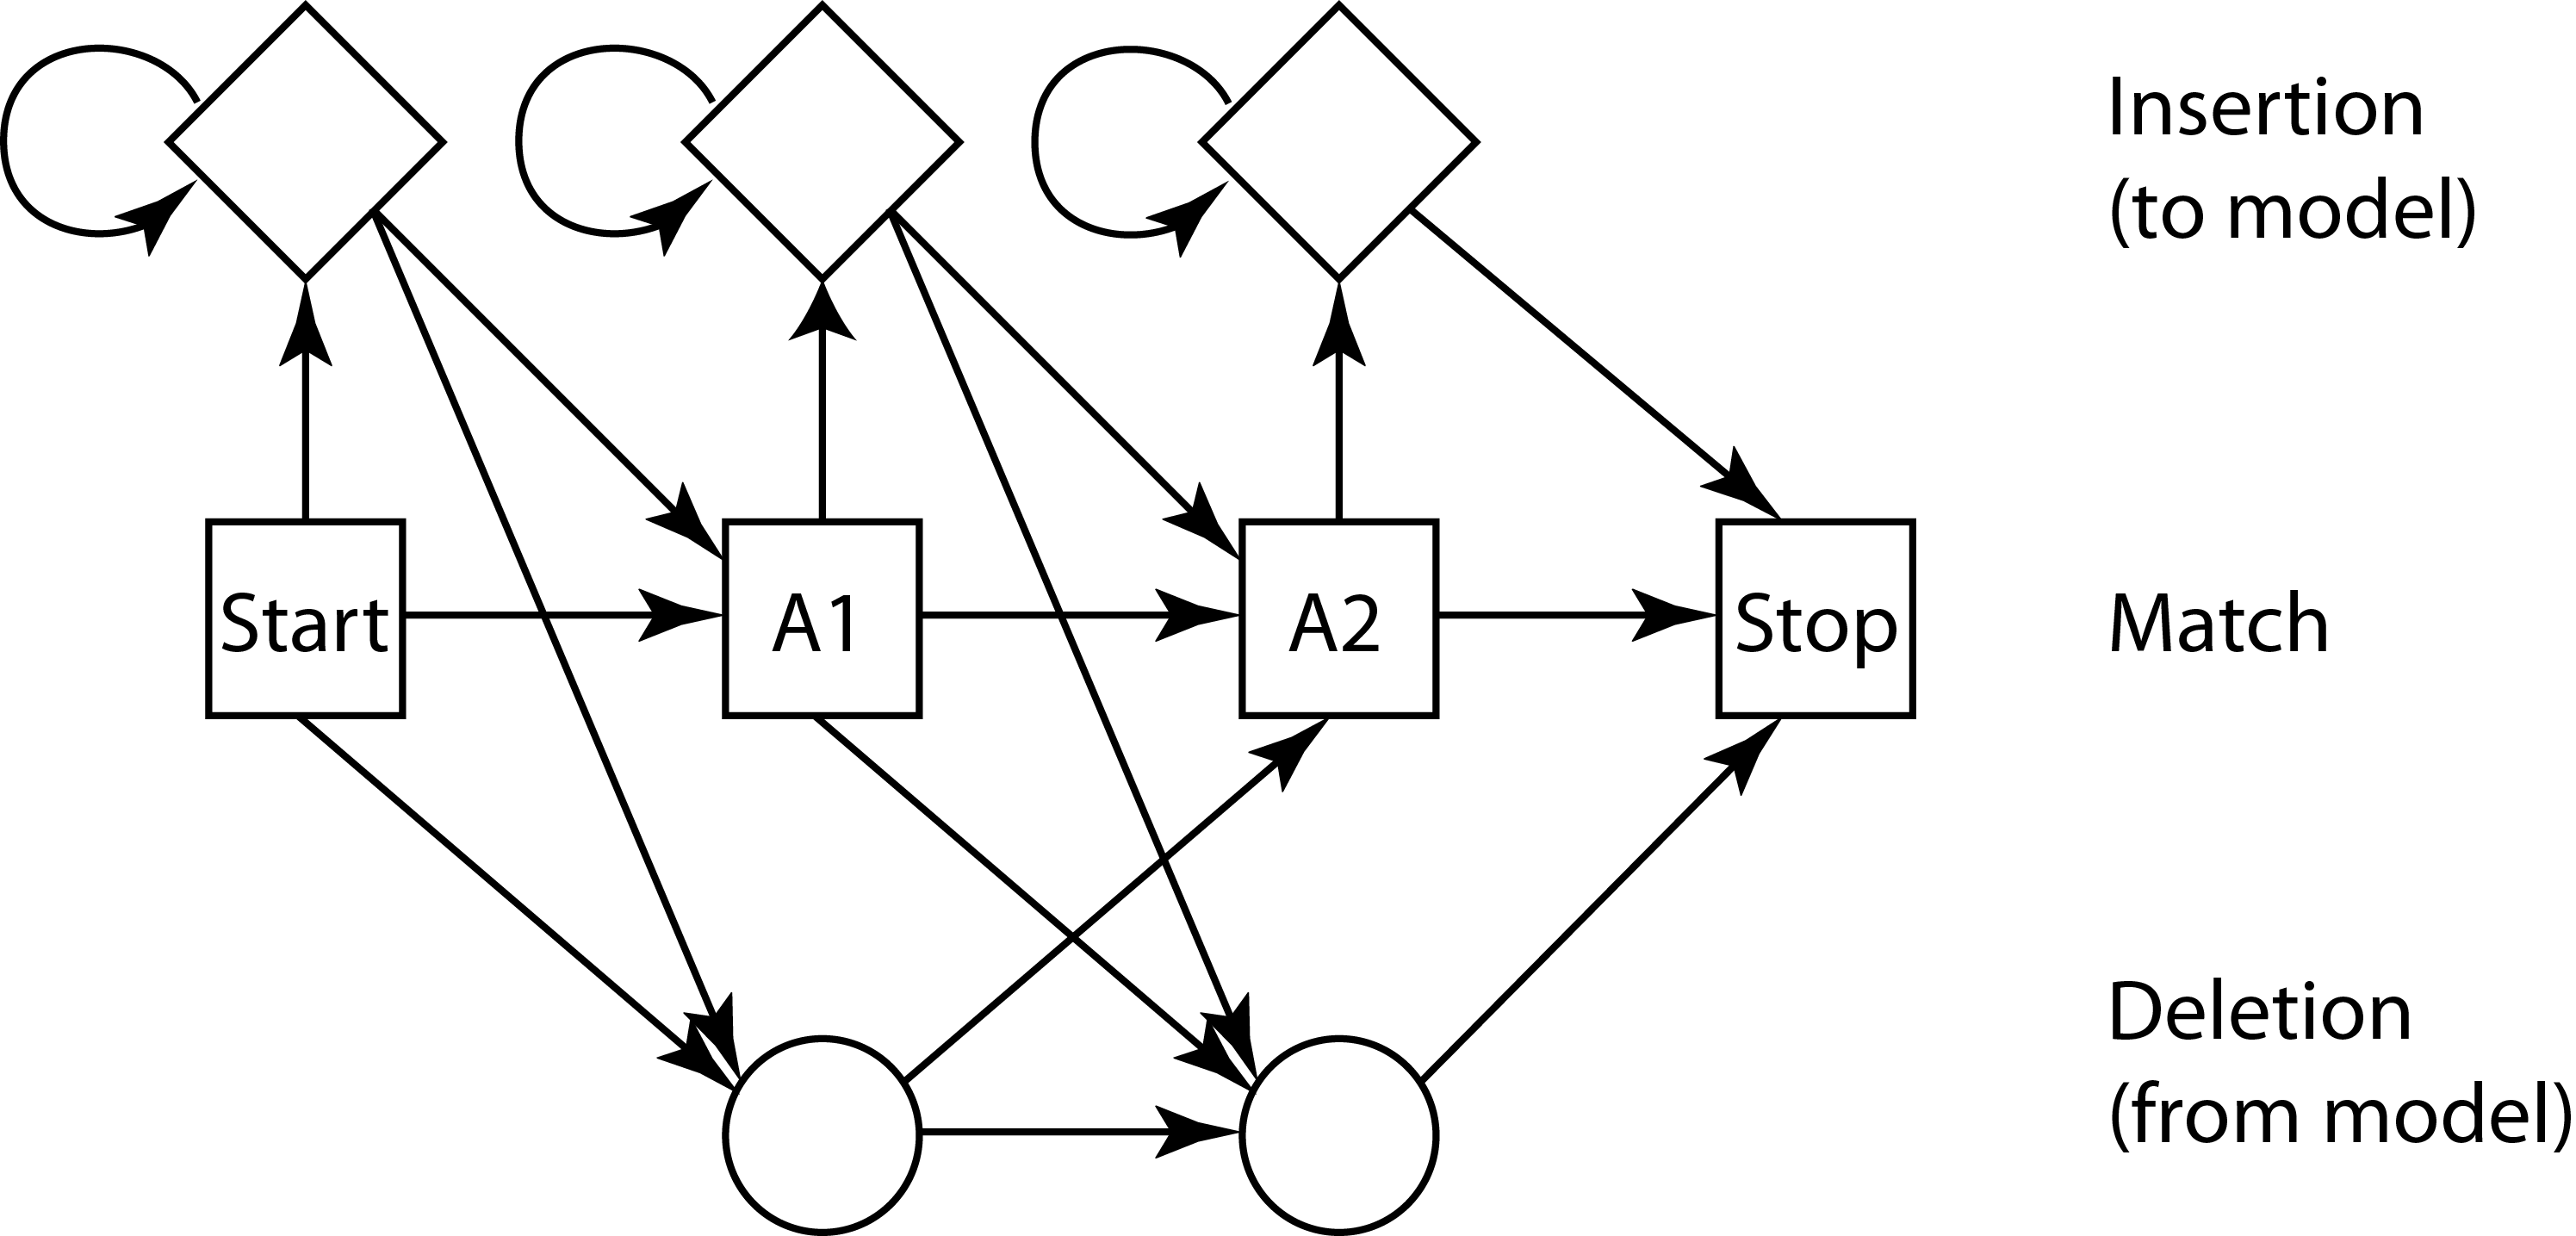
\includegraphics[width=0.5 \textwidth]{fig13/HMM_profile_example_1.png}
  \caption{An HMM for an alignment of two columns A1 and A2}
\end{figure}

%
% Example of HMM profile for finding local alignments
%
\subsubsection*{Example of HMM profile for finding sub-strings}
Assume Seq1 = ’q1 q2 q3 q4’ and its path is indicated with solid lines. Create the alignment of Seq1 and the profile.

\begin{table}[H]
\small
\centering
\begin{tabular}{|l|l|l|l|l|l|}
\hline
   & Start                    & Insertion                & Match                    & Deletion                 & Stop                     \\ \hline
   & -1                       & \cellcolor[HTML]{C0C0C0} & \cellcolor[HTML]{C0C0C0} & \cellcolor[HTML]{C0C0C0} & \cellcolor[HTML]{C0C0C0} \\ \hline
q1 & \cellcolor[HTML]{C0C0C0} & (2 start)                &                          &                          & \cellcolor[HTML]{C0C0C0} \\ \hline
q2 & \cellcolor[HTML]{C0C0C0} &                          & (4 deletion)             & (3 insertion)            & \cellcolor[HTML]{C0C0C0} \\ \hline
q3 & \cellcolor[HTML]{C0C0C0} & (5 match)                &                          &                          & \cellcolor[HTML]{C0C0C0} \\ \hline
q4 & \cellcolor[HTML]{C0C0C0} & (6 Insertion)            &                          &                          & \cellcolor[HTML]{C0C0C0} \\ \hline
   & \cellcolor[HTML]{C0C0C0} & \cellcolor[HTML]{C0C0C0} & \cellcolor[HTML]{C0C0C0} & \cellcolor[HTML]{C0C0C0} & (7 insertion)            \\ \hline
\end{tabular}
\end{table}

\begin{figure}[H]
  \centering
      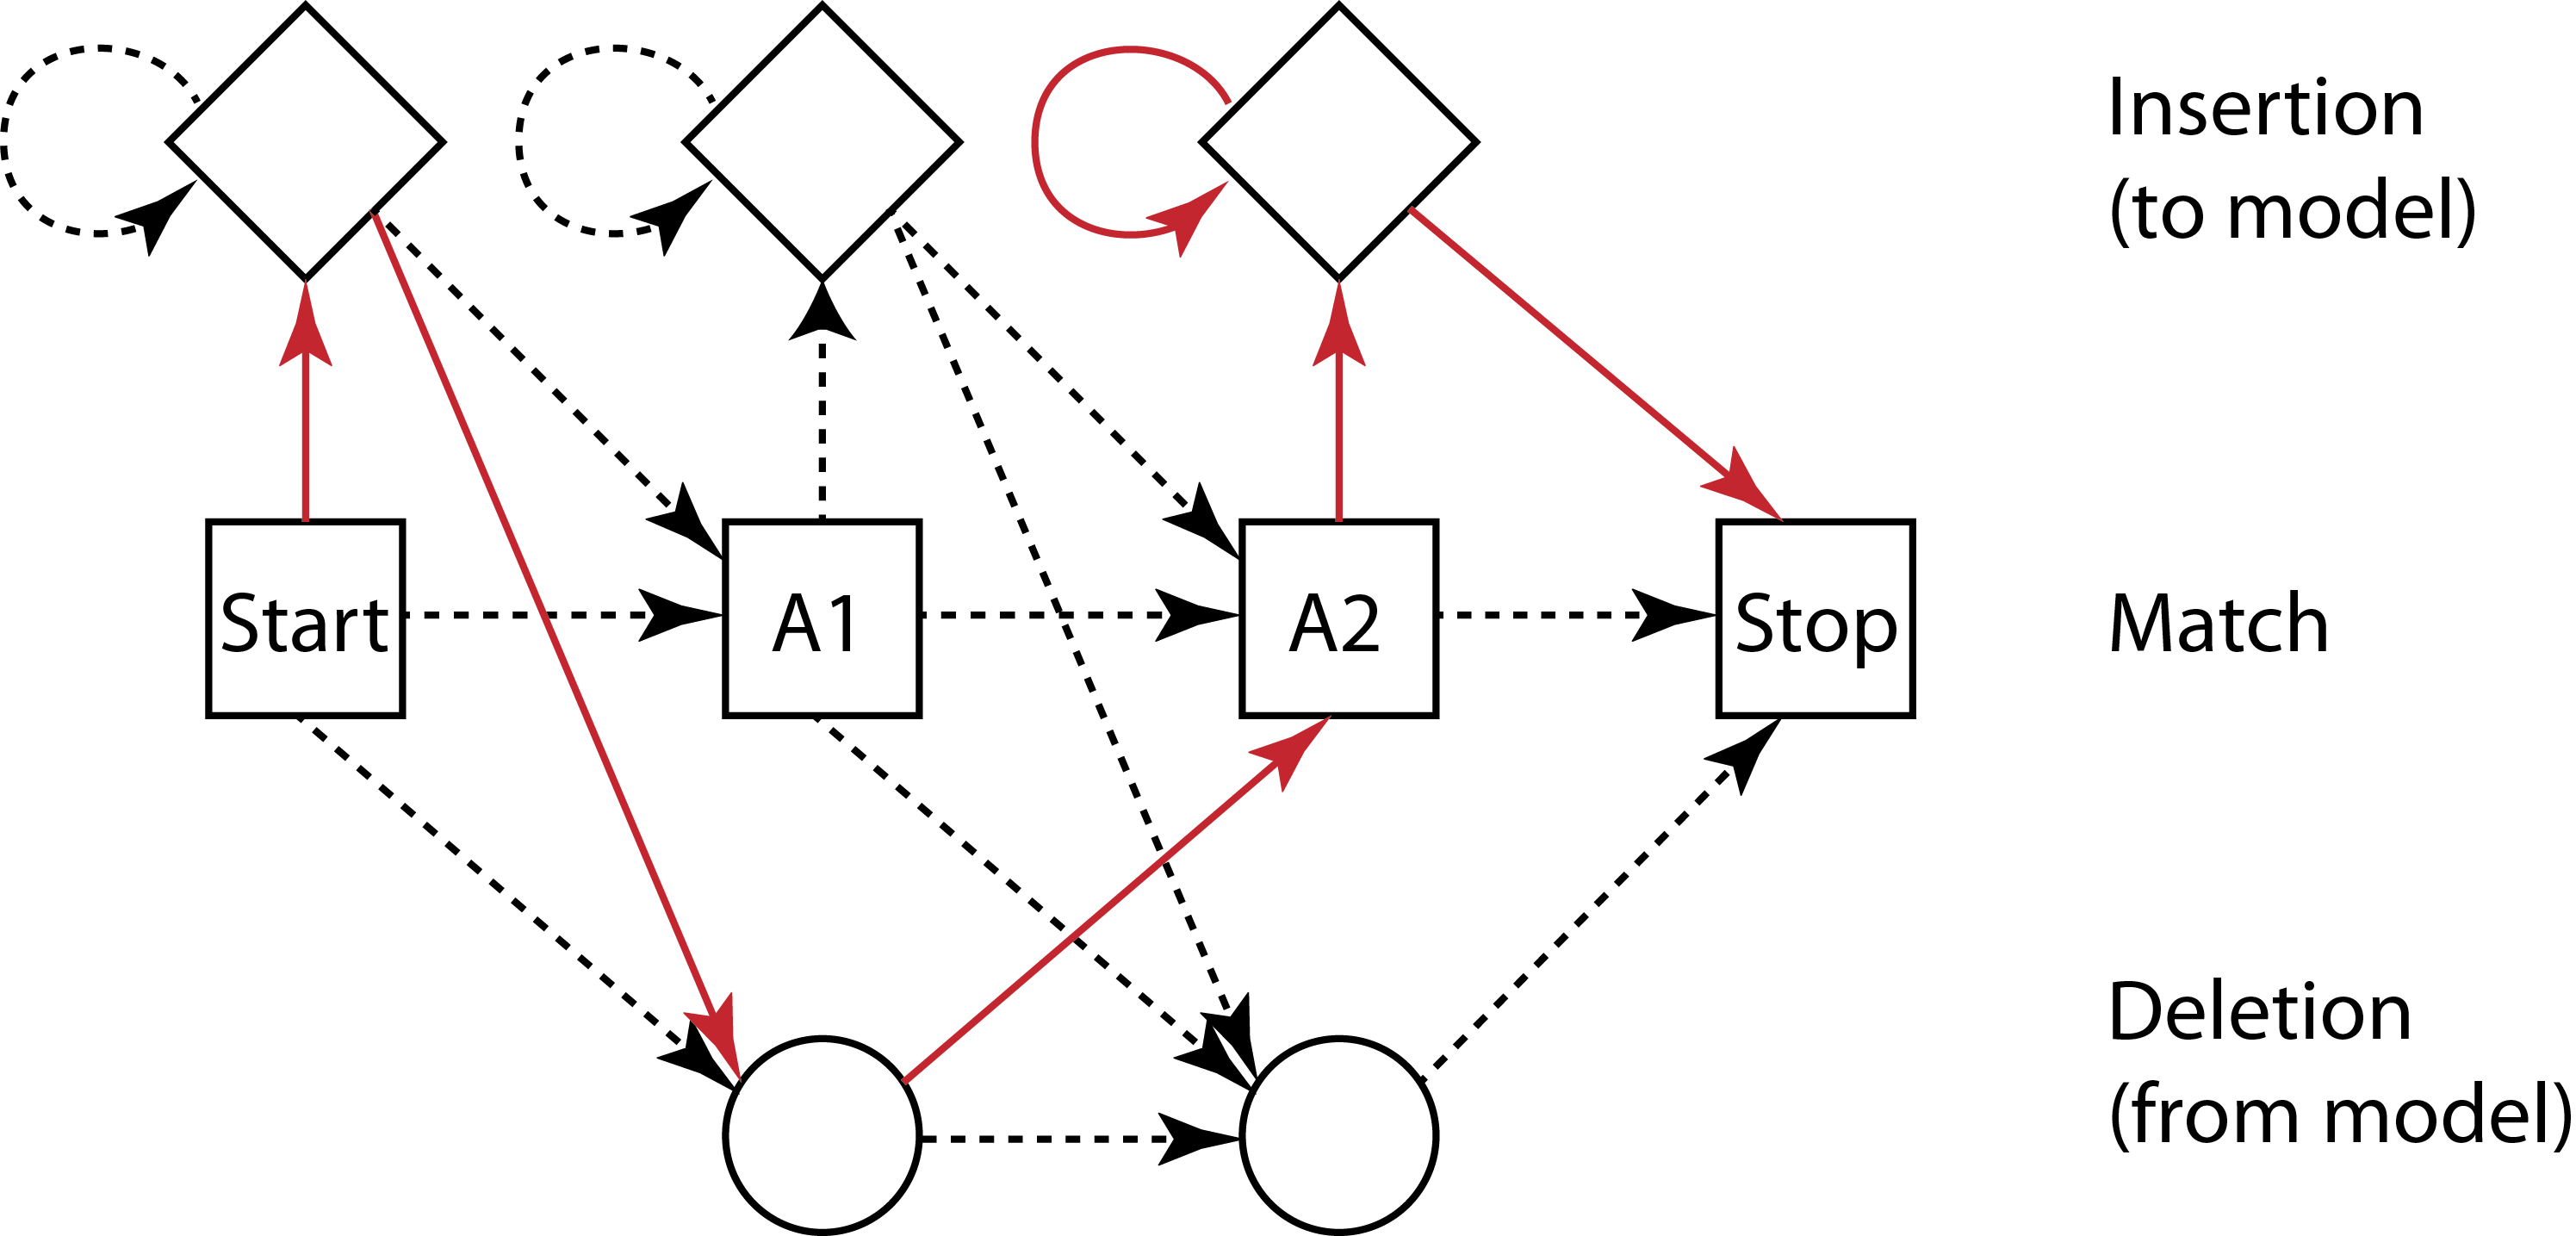
\includegraphics[width=0.5 \textwidth]{fig13/HMM_profile_example_2.png}
  \caption{An HMM profile to find the optimal alignment}
\end{figure}

\noindent
Local alignment:
\begin{verbatim}
   q1  -   q2  q3  q4
   -   A1  A2  -   -
\end{verbatim}

\bigskip 

%\end{document}


\end{document}
